\documentclass[10pt,landscape]{article}
\usepackage[utf8]{inputenc}
% \usepackage[ngerman]{babel}
\usepackage[T1]{fontenc}
%\usepackage[LY1,T1]{fontenc}
%\usepackage{frutigernext}
%\usepackage[lf,minionint]{MinionPro}
\usepackage{tikz}
\usetikzlibrary{shapes,positioning,arrows,fit,calc,graphs,graphs.standard,trees}
\usepackage[nosf]{kpfonts}
\usepackage[t1]{sourcesanspro}
\usepackage{multicol}
\usepackage{wrapfig}
\usepackage[top=7mm,bottom=7mm,left=7mm,right=7mm]{geometry}
\usepackage[framemethod=tikz]{mdframed}
\usepackage{microtype}
\usepackage{pdfpages}
\usepackage{xcolor}
\usepackage{tikz-qtree}
\usepackage{forest}
% \usetikzlibrary{trees,shapes,arrows} 
\usepackage{algpseudocodex}
\usepackage{algorithm2e}
\usepackage{algorithmicx}
\usepackage{scalerel}

% \usepa
% \usepackage{fontspec}

\let\bar\overline

\include{style/def}

\begin{document}
%\footnotesize
\small
\begin{multicols*}{3}
% \input{inhalt/aussagen}
\section{Machine Learning}
\subsection{Types of Learning}
\emph{Supervised Learning:} - learn a model from labeled training data to make predictions about unseen or future data.
\emph{Unsupervised Learning:} - learn a model from unlabeled data to discover hidden patterns or groupings in data.
\emph{Reinforcement Learning:} - develop a system (agent) that improves its performance based on interactions with the environment. maximize reward fucntion.
\subsection{k-Nearest Neighbors}
Given a set of labeled data, classify a new data point based on the majority vote of its k nearest neighbors according to some distance metric such as Euclidean, Manhattan, Minkowski, Hamming, Cosine Similarity. The algorithm for kNN is as follows:
\begin{enumerate}
    \item Compute distance between query point and all examples.
    \item Sort by distance.
    \item Select the k closest examples.
    \item Classify the query point by majority vote.
\end{enumerate}
\subsection{Regression}
Relationship between input and output variables is modeled by fitting a function to the data. Given a set of $n$ labeled pairs $(x_i,y_i)$, find a function $f(x)=\beta_0+\beta_1 x$ that approximates $y$ for a given $x$. We can use the least squares method to find the best fit line using the formula \[\beta_1=\frac{\sum^n_{i=1}(x_i-\bar{x})(y_i-\bar{y})}{\sum^n_{i=1}(x_i-\bar{x})^2}, \beta_0=\bar{y}-\beta_1\bar{x}\].
\subsection{Bayesian Learning}
\subsubsection{Bayes Rule:} $\mathbb{P}(Y=k|X=x) \propto \mathbb{P}(X=x|Y=k)\mathbb{P}(Y=k)$ Classification is like calculating posterior probability, so we can calculate using Bayre's Rule.
\subsubsection{Naive Bayes:} Assume features are independent given class to reduce dimensionality. \(\mathbb{P}(Y=k|\mathbf{X}=\mathbf{x})\propto \prod^{p}_{j=1}\mathbb{P}(X_j=x_j|Y=k)\mathbb{P}(Y=k)\)
If the features are continuous, we can use a Gaussian distribution.
\subsubsection{Laplace Smoothing:} estimate conditional by adding a constant factor that is greater than 0 to each count. \(\mathbb{P}(X_j=c|y)=\frac{n_{c}+\alpha}{n+v}\) where $n_c$ is the number of times $X_j=c$ and $n$ is the number of training examples and $v$ is the number of levels in feature $X_j$.
\subsubsection{Maximum Likelihood Estimation} \textbf{MLE:} estimate parameters of a model by maximizing the likelihood function $\mathcal{L}(\theta|X)$ which is the probability of the observed data $X$ given the model parameters $\theta$. The formula is: \[\hat{\theta}_{MLE}=\underset{\theta}{\text{argmax}}\mathcal{L}(\theta|X)=\underset{\theta}{\text{argmax}}\prod_{i=1}^{n}f(x_i|\theta)\] where $f(x_i|\theta)$ is the probability density function of the $i$th observation.
\subsubsection{Continuous Features:} When given a continuous feature you can use a Gaussian distribution to estimate the probability density function. \[f(x|\mu,\sigma^2)=\frac{1}{\sqrt{2\pi\sigma^2}}e^{-\frac{(x-\mu)^2}{2\sigma^2}}\] where $\mu$ is the mean and $\sigma^2$ is the variance. We can use the data we have to estimate the parameters $\mu$ and $\sigma^2$ using the following formulas: \[\hat{\mu}=\frac{1}{n}\sum_{i=1}^{n}x_i\] \[\hat{\sigma}^2=\frac{1}{n}\sum_{i=1}^{n}(x_i-\hat{\mu})^2\]
\subsubsection{Bayesian Belief Networks:} Directed acyclic graph that represents a set of conditional independence assumptions. For example:
\begin{minipage}[b]{0.2\linewidth}
    \begin{tikzpicture}[scale=.45,transform shape,->,>=stealth',shorten >=1pt,auto,node distance=2cm,
        thick,main node/.style={myblue!80,circle,draw,font=\sffamily\Large\bfseries}]
        \node[main node] (A) at (0,1) {A};
        \node[main node] (X) [below right of=A] {X};
        \node[main node] (B) [above right of=X] {B};
        \node[main node] (C) [below left of=X] {C};
        \node[main node] (D) [below right of=X] {D};
        
        \path[every node/.style={myblue!80,font=\sffamily\small}]
        (A) edge [color=myblue!80] node [above] {} (X)
        (B) edge [color=myblue!80] node [above] {} (X)
        (X) edge [color=myblue!80] node [above left] {} (C)
        edge [color=myblue!80] node [above right] {} (D);
    \end{tikzpicture}
\end{minipage}%
\begin{minipage}[b]{0.76\linewidth}
   \begin{enumerate}
    % \item $\mathbb{P}(A,B,C,D,X)=\mathbb{P}(A)\mathbb{P}(B)\mathbb{P}(C|X)\mathbb{P}(D|X)\mathbb{P}(X|A,B)$
    \item $\mathbb{P}(CD|X)=\mathbb{P}(C|X)\mathbb{P}(D|X)$
    \item $\mathbb{P}(X|AB)=\mathbb{P}(X|AB)$
    \item $\mathbb{P}(\cdot)=\mathbb{P}(A)\mathbb{P}(B)\mathbb{P}(X|AB)\mathbb{P}(C|X)\mathbb{P}(D|X)$
    \item $\mathbb{P}(X|\cdot)\propto\mathbb{P}(A)\mathbb{P}(B)\mathbb{P}(C|X)\mathbb{P}(D|X)$
   \end{enumerate}
\end{minipage}

\section{Decision Trees}
\subsection{Definition:} Decision Trees are a an \emph{interpretable non-parametric supervised learning} method used for classification and regression. Goal: create a model that predicts the value of a target variable by learning simple decision rules inferred from the data features.
\subsection{Regression Trees:} Predict a continuous target variable. The tree is built by splitting the source set into subsets based on an attribute value test. This process is repeated on each derived subset in a recursive manner called recursive partitioning. The recursion is completed when the subset at a node all has the same value of the target variable, or when splitting no longer adds value to the predictions.
\subsubsection{Recursive Binary Splitting:} The process of splitting the data at a node into two groups that lead to the greatest reduction in RSS where $\mathtt{RSS}= \sum_{j=1}^{J}\sum_{i\in R_j}(y_i-\hat{y}_{R_j})^2$ and $\hat{y}_{R_j}=\frac{1}{N_{R_j}}\sum_{i\in R_j}y_i$. \emph{Gain} is the reduction in RSS from the split.
\subsubsection{Cost Complexity Pruning:} The process of pruning a tree to avoid overfitting. We define a subtree $T \subset T_0$ to be any tree that can be obtained by pruning $T_0$ (removing some of its subtrees). We then define the cost complexity criterion to be \[\mathtt{RSS} =\sum_{m=1}^{|T|}\sum_{i:x_i\in R_m}(y_i-\hat{y}_{R_m})^2+\alpha|T|\] where $|T|$ is the number of terminal nodes of $T$, $R_m$ is the rectangle (region) corresponding to the $m$th terminal node, $\hat{y}_{R_m}$ is the predicted response associated with $R_m$, and $\alpha\geq 0$ is a tuning parameter that controls the size of the tree. We seek the subtree that minimizes this equation.
\subsection{Classification Trees:} Predict a categorical target variable. The tree is built by splitting the source set into subsets based on an attribute value test. This process is repeated on each derived subset in a recursive manner called recursive partitioning. The recursion is completed when the subset at a node all has the same value of the target variable, or when splitting no longer adds value to the predictions.
\subsubsection{Classification Error Rate:} (CER) The proportion of training observations in a region that don't belong to the most common class. \[\mathtt{CER}=1-\max(\hat{p}_{mk})\] where $\hat{p}_{mk}$ is the proportion of training observations in the $m$th region that are from the $k$th class. This may not be a good criterion for tree pruning because it is not sufficiently sensitive for tree growing.
\subsubsection{Gini Index:} The Gini index is a measure of total variance across the $K$ classes. \[\mathtt{Gini}=\sum_{k=1}^{K}\hat{p}_{mk}(1-\hat{p}_{mk})\] The Gini index is referred to as a measure of node purity. A small value indicates that a node contains predominantly observations from a single class. The Gini index is used in the \emph{CART} algorithm.
\subsubsection{Cross-Entropy:} The cross-entropy is a measure of total variance across the $K$ classes. A low value for cross entropy indicates that a node contains predominantly observations from a single class.
 \[\mathtt{Cross-Entropy}=-\sum_{k=1}^{K}\hat{p}_{mk}\log{\hat{p}_{mk}}\] where $\hat{p}_{mk}$ is the proportion of training observations in the $m$th region that are from the $k$th class.
The cross-entropy is used in the \emph{C4.5} algorithm.
\subsubsection{Splitting to Maximize Gain:} The process of splitting the data at a node into two groups that lead to the greatest reduction in impurity. \emph{Gain} is the reduction in impurity from the split. \[\mathtt{Gain}=\mathtt{Impurity}_{\text{parent}}-\sum_{j=1}^{\text{children}}\frac{N_j}{N}\mathtt{Impurity}_{\text{child}_j}\] when we select the Gini index as the measure of impurity this is know as \emph{Gain} and with cross-entropy it is known as \emph{Information Gain}.
\subsection{Determining the Best Split:} We can \emph{determine the best split by considering all possible splits for all features and selecting the split that maximizes the gain}. This is computationally expensive so we can use a greedy approach and consider only a subset of the features at each node. We can also use a random forest to select the best split.
\subsection{Ensemble Methods and Boosting:} Ensemble methods are learning algorithms that construct a set of classifiers and then classify new data points by taking a (weighted) vote of their predictions. Boosting is an ensemble method that fits a sequence of weak learners (models that are only slightly better than random guessing) on repeatedly modified versions of the data. The predictions are then combined through a weighted majority vote (classification) or a weighted sum (regression) to produce the final prediction. A common tree boosting algorithm is \emph{AdaBoost}
\section{Fuzzy Logic and Fuzzy Sets}
Similar to probability theory, fuzzy logic is a mathematical framework for representing and reasoning with uncertainty. Fuzzy logic is a superset of conventional (Boolean) logic that has been extended to handle the concept of partial truth -- truth values between ``completely true'' and ``completely false''. Fuzzy logic is used in many applications such as control systems, expert systems, and data mining.
\subsection{Fuzzy Terms:} Given a universe of discourse $U$, a fuzzy set $A\in U$ is defined by a membership function $\mu_A:U\rightarrow[0,1]$.
% \begin{enumerate}
%     \item  $\mu_A(x)$ is the degree of membership of $x\in A$.
%     \item \emph{support} of $A$ set of $x\in U$ s.t. \(\mu_A(x)>0\).
%     \item \emph{core} of $A$ set of $x\in U$ s.t. $\mu_A(x)=1$.
%     \item \emph{height} of $A$ is $\max_{x\in U}\mu_A(x)$.
% \end{enumerate}
Additionally, we define the empty set $\emptyset$ as the fuzzy set with membership function $\mu_{\emptyset}(x)=0$ for all $x\in U$ and the universal set $U$ as the fuzzy set with membership function $\mu_U(x)=1$ for all $x\in U$.
\subsection{Fuzzy Set Operations:}
\textbf{Main Set Operations:}
\begin{enumerate}
        \item \textbf{Complement:} $\mu_{\bar{A}}(x)=1-\mu_A(x)$
        \item \textbf{Union:} $\mu_{A\cup B}(x)=\max(\mu_A(x),\mu_B(x))$
        \item \textbf{Intersection:} $\mu_{A\cap B}(x)=\min(\mu_A(x),\mu_B(x))$
        \item \textbf{Difference:} $\mu_{A\setminus B}(x)=\max(\mu_A(x),1-\mu_B(x))$
\end{enumerate}
The fuzzy set operations for interaction, union, and complement can be defined in terms of the norms and conorms of the membership functions. A \emph{T-norm}, used for fuzzy unions, is binary function \(T:[0,1]\times[0,1]\rightarrow[0,1]\) that satisfies the following conditions:
\begin{enumerate}
    \item $T(x,y)=T(y,x)$ (commutative)
    \item $T(x,1)=x$ (identity)
    \item $x\leq y\Rightarrow T(x,z)\leq T(y,z)$ (monotonic)
    \item $T(x,T(y,z))=T(T(x,y),z)$ (associative)
\end{enumerate}
\emph{T-conorm}, used for fuzzy intersections, is binary function \(S:[0,1]\times[0,1]\rightarrow[0,1]\) that satisfies the following conditions:
\begin{enumerate}
    \item $S(x,y)=S(y,x)$ (commutative)
    \item $S(x,0)=x$ (identity)
    \item $x\leq y\Rightarrow S(x,z)\leq S(y,z)$ (monotonic)
    \item $S(x,S(y,z))=S(S(x,y),z)$ (associative)
\end{enumerate}
\subsection{interpretable Rule Systems:} A rule system is a set of rules of the form \emph{if-then} where the \emph{if} part is called the \emph{antecedent} and the \emph{then} part is called the \emph{consequent}. To design a set of rules for a fuzzy system, we first need to \emph{fuzzify} the inputs using a set of membership functions. Then we apply the rules to the fuzzy inputs to obtain fuzzy outputs. Finally, we \emph{defuzzify} the fuzzy outputs to obtain crisp outputs. The defuzzification process can be done using the \emph{centroid method} or the \emph{max membership method}.
\subsection{Fuzzy Inference Systems:} A fuzzy inference system (FIS) is a system that uses fuzzy rules and fuzzy logic to map inputs to outputs. FIS can be used for modeling complex nonlinear systems. FIS are composed of four main components: a rule base, a database, a fuzzification interface, and a defuzzification interface.
\subsubsection{Firing Level of a Rule:} The firing level of a rule is the degree to which the antecedent of the rule is satisfied. The firing level of a rule is computed by taking the minimum of the membership functions of the antecedent. \[\text{Firing Level}=\min(\mu_{A_1}(x_1),\mu_{A_2}(x_2),\dots,\mu_{A_n}(x_n))\]
\subsubsection{Chopping:} During inference we can use the firing level of a rule to determine the degree to which the consequent is satisfied. The degree to which the consequent is satisfied is computed by taking the minimum of the firing level and the membership function of the consequent. \[\text{Degree of Satisfaction}=\min(\text{Firing Level},\mu_{B}(y))\] We can then ``chop'' the output membership function at the degree of satisfaction which essentially redistributes the membership function to the degree of satisfaction. \[\mu_{B'}(y)=\begin{cases}
    \mu_B(y) & \text{if } \mu_B(y)\leq \text{Firing Level}\\
    \text{Firing Level} & \text{if } \mu_B(y)>\text{Firing Level}\end{cases}\]
\subsubsection{Wang-Mendel Algorithm:} The Wang-Mendel algorithm is a method for generating fuzzy rules from numerical data. The algorithm is as follows: given a set of \(p\) features \(x_1,x_2,\dots,x_p\) and a target variable \(y\), we first partition the input space into a set of fuzzy sets \(A_1,A_2,\dots,A_p\) and the output space into a set of fuzzy sets \(B_1,B_2,\dots,B_q\). Then we compute the membership functions \(\mu_{A_i}(x_i)\) and \(\mu_{B_j}(y)\) for each fuzzy set. Finally, we compute the fuzzy rules using the following formula: \[\mu_{A_i\rightarrow B_j}(x_i,y)=\min(\mu_{A_i}(x_i),\mu_{B_j}(y))\] breaking ties by selecting the rule with the highest confidence level \(\mu_{A_i}(x_i)\). Collect all \emph{if-then} rules with the same antecedent and combine them into a single rule with the consequent being the union of the consequents of the individual rules.
\textbf{Algorithm:} For the exam, determine fuzzy sets where each feature has the highest membership and use these to create a set of \emph{if-then} rules.
\subsubsection{Fuzzy C-Means Clustering (Soft K-Means):} Fuzzy C-Means clustering is a method for clustering data points into \(c\) clusters. Given a set of \(n\) data points \(\mathbf{X}=\{x_1,x_2,\dots,x_n\}\) returns a list of \(c\) cluster centers \(\mathbf{V}=\{v_1,v_2,\dots,v_c\}\) and a partition matrix \(\mathbf{W}=w_{ij}\in [0,1],i=1,2,\dots,n,j=1,2,\dots,c\) where \(w_{ij}\) represents the degree of membership of \(x_i\) in cluster \(c_j\). The algorithm minimizes the objective function \[J_m=\sum_{i=1}^{n}\sum_{j=1}^{c}w_{ij}^m||x_i-v_j||^2\] where \(m\in{[1,\infty)}\) is a weighting exponent and \[w_{ij}=\frac{1}{\sum_{k=1}^c\left(\frac{\Vert x_i - c_j \Vert } {\Vert x_i - c_k \Vert} \right)^{2/(m-1)}}\]
\textbf{Algorithm:} Practically speaking, for the exam we will likely locate the centroid by visual inspection.
\section{Neural Networks}
\subsection{Perceptron:} A perceptron is a single layer neural network that can be used for classification. The perceptron is a linear classifier that uses the \emph{Heaviside step function} as its activation function. The perceptron is trained using the \emph{perceptron learning algorithm} which is a type of \emph{supervised learning}. The perceptron learning algorithm attempts to learn a weights \(\mathbf{W}\) matrix and bias vector \(\mathbf{b}\) that can be used to classify new inputs according to the formula:
\[\hat{y}=\begin{cases}
    1 & \text{if } \mathbf{W}^T\mathbf{x}+\mathbf{b}\geq0\\
    0 & \text{otherwise}
\end{cases}\]
The \textbf{Perceptron Algorithm:}
\begin{enumerate}
    \item Initialize the weights \(\mathbf{W}\) to small random values.
    \item For each training example \((\mathbf{x},y)\) do the following:
    \begin{enumerate}
        \item Predict \(\hat{y}\) using the current weights \(\mathbf{W}\).
        \item Update \(\mathbf{W}^{(t+1)}=\mathbf{W}^{(t)}+\eta(y-\hat{y})\mathbf{x}\)
    \end{enumerate}
    \item Repeat step 2 until convergence.
\end{enumerate}
\subsection{Feedforward Multilayer Perceptron:} A feedforward multilayer neural network is a neural network that consists of an input layer, one or more hidden layers, and an output layer. Below is a diagram of a feedforward multilayer neural network with two hidden layers, each consisting of 5 neurons and an output layer consisting of 2 neurons. This network accepts 4 input features and produces 2 output features. The bias term is omitted for simplicity.
%tikz graph of neural network with one hidden layer
\begin{center}
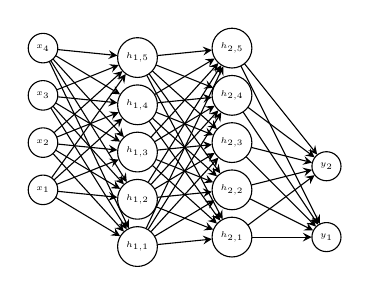
\begin{tikzpicture}[scale=0.6,transform shape,>=stealth,font=\tiny]

% draw input layer
\foreach \i in {1,...,4}
{
  \node[circle,draw=black,minimum size=6mm] (inp\i) at (0,\i) {$x_\i$};
}

% draw hidden layers
\foreach \h in {1,...,5}
{
  \node[circle,draw=black,minimum size=6mm] (hid1\h) at (2,\h-1.2) {$h_{1,\h}$};
  \node[circle,draw=black,minimum size=6mm] (hid2\h) at (4,\h-1) {$h_{2,\h}$};
}

% draw output layer
\foreach \o in {1,2}
{
  \node[circle,draw=black,minimum size=6mm] (out\o) at (6,1.5*\o-1.5) {$y_\o$};
}

% connect input layer to first hidden layer
\foreach \i in {1,...,4}
{
  \foreach \h in {1,...,5}
  {
    \draw[->] (inp\i) -- (hid1\h);
  }
}

% connect first hidden layer to second hidden layer
\foreach \h in {1,...,5}
{
  \foreach \hh in {1,...,5}
  {
    \draw[->] (hid1\h) -- (hid2\hh);
  }
}

% connect second hidden layer to output layer
\foreach \h in {1,...,5}
{
  \foreach \o in {1,2}
  {
    \draw[->] (hid2\h) -- (out\o);
  }
}

\end{tikzpicture}
\end{center}

\subsubsection{Activation Functions:} Activation functions are used to introduce non-linearity into the neural network. The activation function is applied to the weighted sum of the inputs to a neuron. The activation function is typically a non-linear function such as the sigmoid function, the hyperbolic tangent function, or the rectified linear unit (ReLU) function. The sigmoid function is defined as \(\sigma(x)=\frac{1}{1+e^{-x}}\). The hyperbolic tangent function is defined as \(\tanh(x)=\frac{e^x-e^{-x}}{e^x+e^{-x}}\). The ReLU function is defined as \(\text{ReLU}(x)=\max(0,x)\). The ReLU function is typically used in hidden layers and the sigmoid function is typically used in the output layer for binary classification problems. The hyperbolic tangent function is typically used in the output layer for multi-class classification problems.
\subsubsection{Loss Functions:} Loss functions are used to measure the error of the neural network. The loss function is typically a function such as the mean squared error (MSE) function or the cross-entropy function. The cross-entropy function is defined as \(\text{Cross-Entropy}=-\sum_{i=1}^{n}y_i\log{\hat{y}_i}\). The cross-entropy function is typically used in the output layer for classification problems. The MSE function is typically used in the output layer for regression problems. The \emph{MSE function} is defined as \[\text{MSE}=\frac{1}{n}\sum_{i=1}^{n}(y_i-\hat{y}_i)^2\]
\subsubsection{Backpropagation:} At each iteration of training, data is fed through the network until it reaches the output layer. The error is then calculated using the loss function. The error is then propagated backwards through the network using the chain rule to calculate the gradient of the loss function with respect to the weights and biases. The weights and biases are then updated using gradient descent. The process is repeated until convergence. The update equations for gradient descent are as follows:\\
\textbf{Weights:} \[\mathbf{W}^{(t+1)}=\mathbf{W}^{(t)}-\eta\frac{\partial\mathcal{L}}{\partial\mathbf{W}}\] 
\textbf{Biases:} \[\mathbf{b}^{(t+1)}=\mathbf{b}^{(t)}-\eta\frac{\partial\mathcal{L}}{\partial\mathbf{b}}\]
\subsection{Hamming Networks}
Hamming Networks use a feedforward multilayer perceptron architecture followed by a recurrent layer. The recurrent learns prototypes patterns / feature vectors typically present in members of each class. The neuron associated with that prototype indicated the pattern closest to the input.
\subsubsection{The Feedforward Layer:}
The feedforward layer has linear activation function \(\mathbf{f}_{{\scaleto{(1)}{6pt}}}\) is given by: 
\[\mathbf{a}{\scaleto{(1)}{6pt}}=\mathbf{f}_{\scaleto{(1)}{6pt}}\left(\mathbf{W}^T_{\scaleto{(1)}{6pt}}\mathbf{x}+\mathbf{b}_{\scaleto{(1)}{6pt}}\right)\]
The feedforward layer measures the correlation of the input with the prototype each of the prototypes. Input-protype similarity is determined using the matrix \(\mathbf{W}_{\scaleto{(1)}{6pt}}\) where the columns of the matrix are set to be the prototype patterns. Let the prototype patterns be \(\mathbf{p}_1,\mathbf{p}_2,\dots,\mathbf{p}_n\) where \(\mathbf{p}_i\) is the prototype pattern for class \(i\). The matrix \(\mathbf{W}_{\scaleto{(1)}{6pt}}\) and bias vector \(\mathbf{b}_{\scaleto{(1)}{6pt}}\) are defined as:
\[
\mathbf{W}_{\scaleto{(1)}{6pt}}=
    \begin{bmatrix}
        \mathbf{q}_1 & \mathbf{q}_2 & \cdots & \mathbf{q}_K
    \end{bmatrix},\  
        \mathbf{b}_{\scaleto{(1)}{6pt}}=\begin{bmatrix}
            p & p & \cdots & p
    \end{bmatrix}_{K\times 1}^T
\]%
where \(K\) is the number of prototype patterns/classes and is equal to the number of neurons in the first layer \(S_{\scaleto{(1)}{6pt}}\). This choice of \(\mathbf{W}_{\scaleto{(1)}{6pt}}\) and \(\mathbf{b}_{\scaleto{(1)}{6pt}}\) ensures that the output of the first layer is the correlation of the input with each of the prototype patterns because the inner product measures the angles between the prototype vector and the new input, the \(p\) term ensures that the output is positive, and the ReLU function ensures that the output is non-negative. The output of the first layer is then fed into the recurrent layer.\\
\subsubsection{The Recurrent Layer:} The recurrent layer is initialized by the output of the first layer like \( \mathbf{a}_{\scaleto{(1)}{6pt}}(0)= \mathbf{a}_{\scaleto{(1)}{6pt}}\) and then updated according to:
% \begin{minipage}[b]{0.4\linewidth}
    \begin{equation*}
        \mathbf{a}_{\scaleto{(0)}{6pt}}\gets \mathbf{W}^T_{\scaleto{(1)}{6pt}}\mathbf{x}+\mathbf{b}_{\scaleto{(1)}{6pt}},\quad\text{ and }\quad
%     \end{equation*}
% % \end{minipage}%
% % {\hfill\color{gray}\vrule\hfill}%
% % \begin{minipage}[b]{0.5\linewidth}
%     \begin{equation*}
        \mathbf{a}_{\scaleto{(2)}{6pt}}(t+1)=\mathbf{f}_{\scaleto{(2)}{6pt}}
    \left(
        \mathbf{W}^T_{\scaleto{(2)}{6pt}}\mathbf{a}_{\scaleto{(2)}{6pt}}(t)
    \right)
    \end{equation*}
% \end{minipage}%
where \(\mathbf{f}_{\scaleto{(2)}{6pt}}=\max(0,x)\) is the ReLU activation function of the recurrent layer. 

The weight matrix \(\mathbf{W}_{\scaleto{(2)}{6pt}}\) for the recurrent layer is initialized with:
\[
    \mathbf{W}_{\scaleto{(2)}{6pt}}=
        \begin{bmatrix}
            1 &&  -{\scaleto{\epsilon}{9pt}}\\
            &\ddots&\\
            -{\scaleto{\epsilon}{9pt}}&&1
        \end{bmatrix}_{K\times K}
\]
where \(\epsilon < \frac{1}{S-1}\). The feedforward layer acts like an indicator where the most strongly correlated protype transmits the largest signal to the recurrent layer. The recurrent layer then iteratives reapplies the weight matrix until features with lower correlation eventually drop out. Upon convergence, a prediction is made.\\
\begin{center}
\noindent\color{mypink}\rule{4cm}{0.4pt}\\
\emph{\textbf{Neurons that fire together, wire together.}} \\
\(\quad \quad \quad \quad \quad \quad \quad \quad\quad \quad\) - Donald Hebb\\
\noindent\color{mypink}\rule{3cm}{0.4pt}\\
\end{center}
\subsection{Hopfield Networks}
Hopfield networks are a type of recurrent neural network that can be used for classification and optimization. Hopfield networks are composed of a set of neurons that are connected to every other neuron. 
\subsubsection{Recurrent Layer Structure}
The recurrent layer is initialized with the input \(\mathbf{x}\). The structure of the recurrent layer is as follows:
\[\mathbf{a}(0)\gets\mathbf{x},\quad\text{ and }\quad\mathbf{a}(t+1)=\mathbf{f}\left(\mathbf{W}^T\mathbf{a}(t)\right)\]
where \(\mathbf{f}\) is the activation function of the recurrent layer. The activation function of the recurrent layer is typically the sign function, hyperbolic tangent function, or the \emph{saturated linear function (SLF)} which is defined as:
\[\texttt{SLF}(n)=\begin{cases}
    1 & \text{if } n\geq 1\\
    n & \text{if } 0\leq n\leq 1\\
    0 & \text{otherwise}
\end{cases}\]
The weight matrix \(\mathbf{W}\) is initialized with \(K\) prototype patterns \(\mathbf{q}_1,\mathbf{q}_2,\dots,\mathbf{q}_K\) where \(\mathbf{q}_k\) is the prototype pattern for class \(k\). The weight matrix \(\mathbf{W}\) is defined as:
\[\mathbf{W}=\sum_{k=1}^K\mathbf{q}_k{\mathbf{q}}_k^T\]
where \(k\) is the class of the prototype pattern and \(K\) is the number of neurons in the network. The result is a square weight matrix \(\mathbf{W}\in\mathbb{R}^{K\times K}\). The iterative process for classification in the recurrent network is as follows:
\[\mathbf{a}(0)\gets\mathbf{x}\] 
\[\implies\quad\mathbf{a}(t+1)=\texttt{SLF}\left(\sum_{k=1}^K\mathbf{q}_k({\mathbf{q}_k}^T\mathbf{x})\right)\]
The quantity scalar quantity \(\alpha_k=\mathbf{q}_k^T\mathbf{x}\) is the correlation of the input with the prototype pattern \(\mathbf{q}_k\). The recurrent process is repeated until the output converges. The output of the network is the class of the prototype pattern that the input is most correlated with. 
\subsection{Supervised Hebbian Learning}
Supervised Hebbian learning is a type of supervised learning that is based on the idea that when neurons on both sides of a synapse are activated, the synapse is strengthened. 
\subsubsection{Linear Associator}
A linear associators is an example of a neural network called an associative memory. The goal of the associator is to learn \(K\) prototype input-output vectors that satisfy:
\[\mathbf{a}=\mathbf{W}^T\mathbf{x}\]
The network should recall input-output pairs it has encouneter and also remain \emph{robust} by ensuring that a small amount of noise to the input only results in a small shift in the prediction.
\subsubsection{The Supervised Hebbian Learning Algorithm}
We initialize the weight matrix \(\mathbf{W}=0\) and then update the weight matrix using the following iterative process:
\emph{\textbf{for each training example \((\mathbf{x}_k,\mathbf{y}_k)\) do the following:}}
\[
    \mathbf{W}^{{\scaleto{(\text{new})}{6pt}}}\gets\mathbf{W}^{{\scaleto{(\text{old})}{6pt}}}+\mathbf{x}_k\mathbf{y}_k^T    
\]
\section{Reinforcement Learning}
The goal of any \emph{reinforcement learning} task is to learn an optimal \emph{policy} \(\pi : S \to A\) that maps the state of the environment to actions so as to maximize the expected \emph{reward}. The agent learns by interacting with the environment. The agent receives a reward $r_t$ and observes the next state $s_{t+1}$ after taking an action $a_t$ in state $s_t$. The agent's goal is to optimize for the \emph{total future discounted reward} which is given by:
\[
    V^\pi(s) = \sum_{t=0}^\infty \gamma^t r_t,\quad 0\leq \gamma < 1
\]
Given an optimal value function $V^*(s)$, the optimal policy $\pi^*(s)$ is given by:
\[
    \pi^*(s) = \text{arg}\max_a \left[r(s,a) + \gamma V^*\left(\delta(s,a)\right)\right]
\]
Many ways to solve this policy optimization problem when all else is know but in unknown environment we must learn \(\delta\) and \(r\).\\
\subsection{Q-Function}
The \emph{Q-function} is a function of the state and action that gives the expected total future discounted reward for taking action $a$ in state $s$ and following policy $\pi$ thereafter. The optimal Q-function is given by:
\[
    Q(s,a) = r(s,a) + \gamma V^*\left(\delta(s,a)\right)
\]
where $r(s,a)$ is the reward for taking action $a$ in state $s$ and $\delta(s,a)$ is the next state after taking action $a$ in state $s$. The optimal policy is given by:
\[
    \pi^*(s) = \text{arg}\max_a Q(s,a)
\]
\subsubsection{Q-Learning}
The learner represents the hypothesis space as a table of Q-values indexed by state and action. The learner interacts with the environment by taking actions and observing the next state and reward. The learner updates the Q-values values in the table using the following update rule:
\[
    \hat{Q}(s_t,a) \gets r + \gamma \max_{a^\prime} \hat{Q}(s_{t+1},a^\prime)
\]
This equation continuously estimates the optimal Q-function by bootstrapping from the current estimate of the optimal Q-function. The learner selects actions using an $\epsilon$-greedy policy. The learner continues to interact with the environment until convergence.
\emph{\textbf{Q-Learning Algorithm:}}
\begin{enumerate}
    \item Initialize Q-values $\hat{Q}(s,a)$ arbitrarily.
    \item Observe current state $s_t$.
    \item Repeat forever:
    \begin{enumerate}
        \item Select action $a_t$ using %$\epsilon$-greedy policy.
        \item Observe reward $r_t$ and next state $s_{t+1}$.
        \item Update Q-values using the update rule. (listed above)
        \item $s_t \gets s_{t+1}$.
    \end{enumerate}
\end{enumerate}
\subsubsection{Exploration:}
The Q-Learning algorithm is ambiguous to the action selection process. The $\epsilon$-greedy policy is a simple way to balance exploration and exploitation. The $\epsilon$-greedy policy selects a random action with probability $\epsilon$ and the greedy action with probability $1-\epsilon$. Another policy allows us to rely on the Q-values to select actions using our trust in Q to determine the probability that we follow Q's hypothesis. \emph{State Transition Updates} during exploration \(\hat{Q}(s,a)\) reward values are only updated when we encounter a non-zero rewaerd.

% \subsubsection{Stochastic Environments:}
% In stochastic environments, the reward and next state are not deterministic. The Q-Learning algorithm can be modified to handle stochastic environments by maximizing the expected Q-value:
% \[
%     \hat{Q}(s_t,a) \gets r + \gamma \mathbb{E}_{a^\prime \sim \pi} \left[\hat{Q}(s_{t+1},a^\prime)\right]
% \]
\begin{center}
    \emph{\textbf{Grid World Example:}}\\
    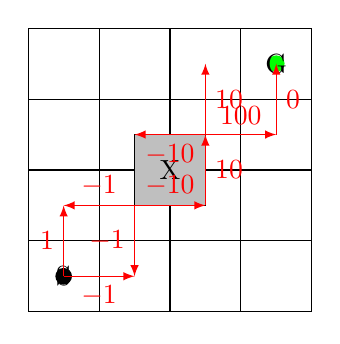
\begin{tikzpicture}[scale=0.9]
        % Draw vertical lines
        \draw (0,0) -- (0,4);
        \draw (1,0) -- (1,4);
        \draw (2,0) -- (2,4);
        \draw (3,0) -- (3,4);
        \draw (4,0) -- (4,4);
        % Draw horizontal lines
        \draw (0,0) -- (4,0);
        \draw (0,1) -- (4,1);
        \draw (0,2) -- (4,2);
        \draw (0,3) -- (4,3);
        \draw (0,4) -- (4,4);
        % Draw start and goal
        \node[circle,fill=black, inner sep=0pt,minimum size=6pt] (start) at (0.5, 0.5) {};
        \node[circle,fill=green, inner sep=0pt,minimum size=6pt] (goal) at (3.5, 3.5) {};
        % Draw obstacles
        \filldraw[fill=gray!50!white, draw=black] (1.5,1.5) rectangle (2.5,2.5);
        % Label cells
        \node at (0.5,0.5) {S};
        \node at (3.5,3.5) {G};
        \node at (2,2) {X};
        % Add Q reward predictions with arrows
        \draw[-latex, red] (0.5,0.5) -- (0.5,1.5) node[midway, left] {$1$};
        \draw[-latex, red] (0.5,0.5) -- (1.5,0.5) node[midway, below] {$-1$};
        \draw[-latex, red] (1.5,1.5) -- (2.5,1.5) node[midway, above] {$-10$};
        \draw[-latex, red] (2.5,1.5) -- (2.5,2.5) node[midway, right] {$10$};
        \draw[-latex, red] (1.5,1.5) -- (1.5,0.5) node[midway, left] {$-1$};
        \draw[-latex, red] (1.5,1.5) -- (0.5,1.5) node[midway, above] {$-1$};
        \draw[-latex, red] (2.5,2.5) -- (3.5,2.5) node[midway, above] {$100$};
        \draw[-latex, red] (3.5,2.5) -- (3.5,3.5) node[midway, right] {$0$};
        \draw[-latex, red] (2.5,2.5) -- (2.5,3.5) node[midway, right] {$10$};
        \draw[-latex, red] (2.5,2.5) -- (1.5,2.5) node[midway, below] {$-10$};
    \end{tikzpicture}
\end{center}






\section{Unsupervised Learning}
In the \emph{unsupervised learning} setting, the agent is given a set of unlabeled data and the goal is to discover hidden patterns or groupings in the data. Common unsupervised tasks include \emph{principal component analysis}, \emph{clustering}, and \emph{density estimation}.
% \emph\textbf{{Principal Component Analysis}}
% Uses properties of the covariance matrix to find the direction of maximum variance in the data. The first principal component is the direction of maximum variance. The second principal component is the direction of maximum variance orthogonal to the first principal component. The $k$th principal component is the direction of maximum variance orthogonal to the first $k-1$ principal components.
\emph\textbf{{Clustering}}
Broad claass of methods which aim to classify or discover sub-groups in the data.
\emph{\textbf{hierarchical clustering:}} no assumption about the number of clusters, usually represented as a dendrogram which is a tree-like diagram that records the sequences of merges or splits for different \(k\) values.

\subsection{K-Means Clustering}
A partion of the data: \(C_1,C_2,\dots,C_k\) must satisfy the constraints that \(C_i\cap C_j=\emptyset\) and \(\bigcup_{i=1}^{k}C_i=\mathbf{X}\). The goal is to minimize variation within clusters. One approach is to minimize the within-cluster sum of squares (WCSS) which is given by \(\sum_{i=1}^{k}\sum_{x\in C_i}||x-\mu_i||^2\) where \(\mu_i\) is the mean of cluster \(C_i\). Another is to minimize the Euclidean distance between each point and its cluster center which is given by \(\mathtt{WCV}(C_k)=\frac{1}{\vert C_k \vert}\sum_{i,i'\in C_k}\sum_{j=1}^P(x_{ij}-x_{i'j})^2\)  where \(C_k\) is the \(k\)th cluster and \(P\) is the number of features. We then seek to minimize:
\[
     \underset{C_1,\dots,C_k}{\mathtt{minimize}}\left\{\sum_{k=1}^{K}\frac{1}{|C_k|}\sum_{i,i'\in C_k}\sum_{j=1}^P(x_{ij}-x_{i'j})^2\right\}
\]
\subsubsection{K-Means Algorithm}
\begin{enumerate}
    \item Randomly assign a number, from 1 to $k$, to each of the data points. These numbers represent the cluster assignments for the observations.
    \item Iterate until the cluster assignments stop changing:
    \begin{enumerate}
        \item For each of the $k$ clusters, compute the cluster centroid. The $k$th cluster centroid is the vector of the $p$ feature means for the observations in the $k$th cluster.
        \item Assign each observation to the cluster whose centroid is closest (where closest is defined using Euclidean distance).
    \end{enumerate}
\end{enumerate}

% \input{inhalt/mengen}
% \input{inhalt/relationen}
% \input{inhalt/abbildungen}
% \input{inhalt/beweise} 
% \input{inhalt/graphen}
%\input{inhalt/graphalgo}
%\input{inhalt/bool}
%\input{inhalt/formeln}
\end{multicols*}
\end{document}